\subsubsection{UC14 - Gestione ordini}
\begin{figure}[h]
	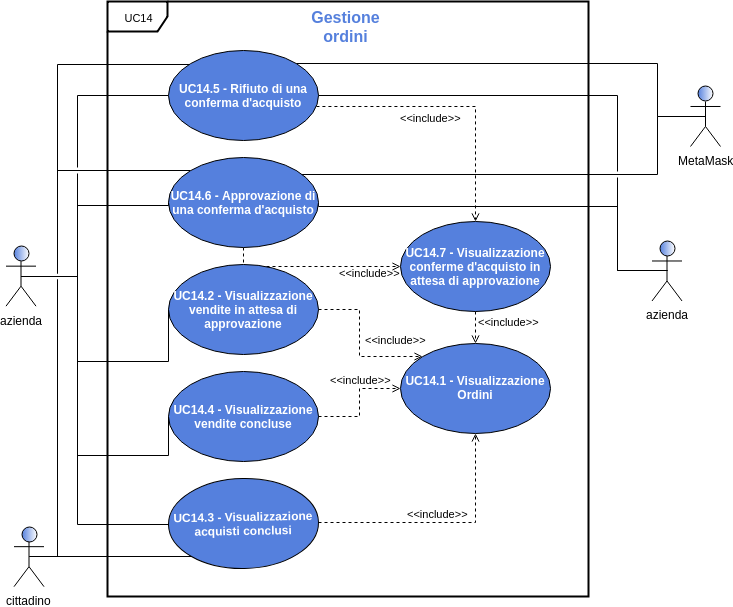
\includegraphics[width=10cm]{res/images/UC14-GestioneOrdini.png}
	\centering
	\caption{Gestione degli ordini}
\end{figure}
\begin{itemize}
	\item \textbf{Attori Primari}: azienda, cittadino;
	\item \textbf{Descrizione}: agli utenti sono messe a disposizione diverse operazione per visualizzare e gestire gli ordini;
	\item \textbf{Scenario principale}: l'utente visualizza e svolge alcune operazioni per gestire gli ordini dei quali ne è partecipe;
	\item \textbf{Precondizione}: il sistema ha riconosciuto l'utente autenticato come azienda o cittadino e mette a disposizione tutte le pagine necessarie alla visualizzazione e gestione degli ordini;
	\item \textbf{Postcondizione}: l'utente ha visualizzato e/o gestito i propri ordini.
\end{itemize} 
\subsubsection{UC14.1 - Visualizzazione ordini}
\begin{itemize}
	\item \textbf{Attori Primari}: azienda, cittadino;
	\item \textbf{Descrizione}: alle aziende ed ai cittadini sono messe a disposizione diverse operazioni per visualizzare e gestire gli ordini all'interno della piattaforma. \`E reso possibile avere un elenco dettagliato di tutti gli ordini, in particolare per ognuno di essi è presente la visualizzazione:
	\begin{itemize}
		\item della data dell'ordine;
		\item del numero dell'ordine;
		\item dei prodotti inclusi nell'ordine [UC5];
		\item totale IVA;
		\item prezzo lordo\glo;
		\item indirizzo di spedizione;
	\end{itemize}
	\item \textbf{Scenario principale}: l'utente visualizza gli ordini per poi poterli gestire;
	\item \textbf{Inclusioni}:
	\begin{itemize}
		\item \textbf{UC5}: visualizzazione dei beni;
	\end{itemize}
	\item \textbf{Precondizione}: il sistema ha riconosciuto l'utente autenticato come azienda o cittadino e mette a disposizione tutte le pagine necessarie alla visualizzazione e gestione degli ordini;
	\item \textbf{Postcondizione}: l'utente ha visualizzato l'elenco dei propri ordini.
\end{itemize} 

\subsubsection{UC14.2 - Visualizzazione vendite in attesa di approvazione}
\begin{itemize}
	\item \textbf{Attori Primari}: azienda;
	\item \textbf{Descrizione}: all'azienda ha la possibilità di visualizzare le vendite effettuate ad altre aziende, che sono in attesa di approvazione;
	\item \textbf{Scenario principale}: l'utente visualizza le vendite in attesa di approvazione tramite una vista dettagliata che include la visualizzazione di: 
		\begin{itemize}
		\item le informazioni dell'ordine [UC14.1];
		\item della data ultima per l'approvazione;
		\item nome azienda-cliente;
		\item partita IVA dell'azienda-cliente;
		\end{itemize}
		\item \textbf{Inclusioni}:
	\begin{itemize}
		\item \textbf{UC14.1}: Visualizzazione degli ordini;
	\end{itemize}
	\item \textbf{Precondizione}:l'utente visita la pagina per la visualizzazione delle vendite che sono in attesa di approvazione;
	\item \textbf{Postcondizione}: l'utente ha visualizzato le proprie vendite in attesa di approvazione.
\end{itemize} 

\subsubsection{UC14.3 - Visualizzazione acquisti conclusi}
\begin{itemize}
	\item \textbf{Attori Primari}: cittadino, azienda;
	\item \textbf{Descrizione}: l'utente può visualizzare la lista degli acquisti conclusi;
	\item \textbf{Scenario principale}: l'utente visualizza la lista degli acquisti conclusi, che hanno un campo aggiuntivo, ovvero la data di conferma dell'ordine;
	\item \textbf{Inclusioni}:
	\begin{itemize}
		\item \textbf{UC14.1}: Visualizzazione degli ordini;
	\end{itemize}
	\item \textbf{Precondizione}: l'utente sta visitando la pagina contenente la lista degli acquisti conclusi;
	\item \textbf{Postcondizione}: l'utente visualizza la lista degli acquisti conclusi.
\end{itemize}

\subsubsection{UC14.4 - Visualizzazione vendite concluse}
\begin{itemize}
	\item \textbf{Attori Primari}: azienda;
	\item \textbf{Descrizione}: l'utente può visualizzare la lista delle proprie vendite ritenute concluse;
	\item \textbf{Scenario principale}: l'utente visualizza la lista delle vendite concluse, che hanno un campo aggiuntivo, ovvero la data di conferma dell'ordine da parte dell'azienda-cliente;
	\item \textbf{Inclusioni}:
	\begin{itemize}
		\item \textbf{UC14.1}: Visualizzazione degli ordini;
	\end{itemize}
	\item \textbf{Precondizione}: il sistema ha riconosciuto l'utente autenticato come azienda e questo ha espresso la volontà di visualizzare la lista delle vendite concluse;
	\item \textbf{Postcondizione}: l'utente visualizza tale lista.
\end{itemize}


\subsubsection{UC14.5 - Rifiuto di una conferma d'acquisto}
\begin{itemize}
	\item \textbf{Attori Primari}: azienda;
	\item \textbf{Attori Secondari}: MetaMask\glo, azienda;
	\item \textbf{Descrizione}: l'azienda può rifiutare una conferma d'acquisto\glo. Per effettuare l'operazione verrà utilizzato MetaMask\glo;
	\item \textbf{Scenario principale}: l'utente visualizza una conferma d'acquisto che necessita di approvazione e decide di rifiutarla;
	\item \textbf{Inclusioni}: 
	\begin{itemize}
		\item \textbf{UC14.7}: visualizzazione delle conferme d'acquisto relative agli acquisti in attesa di approvazione;
	\end{itemize}
	\item \textbf{Precondizione}: il sistema ha riconosciuto l'utente autenticato come azienda ed ha mostrato la lista delle proposte d'acquisto che necessitano di conferma;
	\item \textbf{Postcondizione}: l'azienda ha rifiutato la proposta d'acquisto. La proposta non sarà più presente nella lista di attesa per la conferma. Il sistema ritorna l'ammontare trattenuto per l'ordine all'azienda-cliente.
\end{itemize}
\subsubsection{UC14.6 - Approvazione di una conferma di acquisto}
\begin{itemize}
	\item \textbf{Attori Primari}: azienda;
	\item \textbf{Attori Secondari}: MetaMask\glo, azienda;
	\item \textbf{Descrizione}: l'azienda accetta la proposta d'acquisto ricevuta;
	\item \textbf{Scenario principale}: l'azienda decide di approvare una proposta d'acquisto da parte di un acquirente. L'utente acquirente ha la possibilità di effettuare il versamento all'azienda-venditrice;
	\item \textbf{Scenario alternativo}: l'azienda non ha né confermato né approvato la conferma d'acquisto entro la data ultima per l'approvazione;
		\item \textbf{Inclusioni}: 
	\begin{itemize}
		\item \textbf{UC14.7}:  visualizzazione delle conferme d'acquisto relative agli acquisti in attesa di approvazione;
	\end{itemize}
	\item \textbf{Precondizione}: 
	\begin{enumerate}[label=\alph*.]
		\item il sistema ha riconosciuto l'utente autenticato come azienda, e questo ha espresso la volontà di approvare una richiesta d'acquisto;
		\item è stata superata la data ultima per l'approvazione della conferma d'ordine\glo;
	\end{enumerate}
	\item \textbf{Postcondizione}: il suddetto ordine risulta approvato dall'azienda.
\end{itemize}


\subsubsection{UC14.7 - Visualizzazione conferme d'acquisto in attesa di approvazione}
\begin{itemize}
	\item \textbf{Attori Primari}: azienda;
	\item \textbf{Descrizione}: l'azienda può visualizzare delle proposte d'acquisto che necessitano di conferma. Esse sono relative agli acquisti che ha effettuato ma non ancora confermato;
	\item \textbf{Scenario principale}: l'utente visualizza la lista delle proposte d'acquisto che necessitano di conferma. Per ognuna di esse ha a possibilità di confermare la proposta [UC14.6] o di rifiutarla [UC14.5];
	\item \textbf{Inclusioni}:
	\begin{itemize}
		\item \textbf{UC14.1}: Visualizzazione degli ordini;
	\end{itemize}
	\item \textbf{Precondizione}: il sistema ha riconosciuto l'utente autenticato come azienda e questo ha espresso la volontà di visualizzare la lista delle proposte d'acquisto che necessitano di conferma;
	\item \textbf{Postcondizione}: l'azienda visualizza tale lista.
\end{itemize}





